\documentclass[10pt,a4paper]{article}

\usepackage[utf8]{inputenc}
\usepackage[T1]{fontenc}

%%%%%%%%%%% Own packages
\usepackage[a4paper, margin=1in]{geometry}
\usepackage{multicol}
\usepackage{lipsum}
\usepackage{natbib}

% Header/footer
\usepackage{fancyhdr}
\pagestyle{fancy}
\renewcommand{\headrulewidth}{0pt}

% Footnotes at bottom of page
\usepackage[bottom,marginal]{footmisc}
% \setlength{\footnotemargin}{1.8em}

% Maths
\usepackage{physics}
\usepackage{esdiff}
\usepackage{cancel}
\usepackage{amstext,amsbsy,amssymb,mathtools}
\usepackage{times} 
\usepackage{siunitx}
\usepackage{tensor}

%% Graphics
\usepackage{caption}
\captionsetup{margin=20pt,font=small,labelfont=bf}
%\renewcommand{\thesubfigure}{(\alph{subfigure})} % Style: 1(a), 1(b)
%\pagestyle{empty}
\usepackage{graphicx} % Include figure files

% Listsings and items
\usepackage[page]{appendix}
\usepackage[shortlabels]{enumitem}
\setenumerate{wide,labelwidth=!, labelindent=0pt}
\usepackage{varioref}
\usepackage{hyperref}
\usepackage{cleveref}

% Paragraph indent and skip
\setlength{\parindent}{2em}
\setlength{\parskip}{1em}
\setlength\extrarowheight{5pt}

%% User units
\DeclareSIUnit \parsec {pc}

%% User commands
\providecommand{\qwhere}
{%
\ensuremath{
,\quad \text{where} \quad%
}
}
\providecommand{\rCDM}
{\ensuremath{
\textrm{CDM}
}
}

\providecommand{\gtilde}
{
  \ensuremath{
    \tilde{g}
  }
}

\providecommand{\hprime}
{
  \ensuremath{
    \mathcal{H}
  }
}

\allowdisplaybreaks
\title{AST5220 Cosmology \rm{II}\\ 
\vspace{5mm}Milestone 4 - Computing the CMB Power Spectrum}
\author{Jakob Borg}
%%%%%%%
\begin{document}
%%%%%%%
\maketitle
\lhead{Milestone 4 AST5220}
\rhead{Jakobbor}
%%%%%%%%

\section{Introduction}
\label{sec:Introduction}
This is the final milestone of our four part project to compute the cosmic microwave background (CMB) power spectrum, expressed through $C_\ell$. Here we build upon the results from the three previous milestone where we computed the background evolution and expansion of the Universe \citep{milestone1}, the ionization history, the optical depth and visibility function \citep{milestone2} and last the evolution of the perturbations set up by inflation \citep{milestone3}.


The full project can be found on GitHub, here are link to the \href{https://github.com/Lilleborg/AST5220-Cosmology2/tree/master/Numerical_projects}{projects main directory}\footnote{URL: \url{https://github.com/Lilleborg/AST5220-Cosmology2/tree/master/Numerical_projects}}. All computation and calculations are done in "C++", with the source code found \href{https://github.com/Lilleborg/AST5220-Cosmology2/tree/master/Numerical_projects/src}{here}\footnote{URL: \url{https://github.com/Lilleborg/AST5220-Cosmology2/tree/master/Numerical_projects/src}}. 
The main calculations for this milestone may be found in \textit{PowerSpectrum.h}, building upon everything we have done so far. As mentioned in \cite{milestone3} we will need one specific quantity, the source function, which we will implement in the code from the last milestone in \textit{Perturbations.h}.


%  _______ _                           
% |__   __| |                          
%    | |  | |__   ___  ___  _ __ _   _ 
%    | |  | '_ \ / _ \/ _ \| '__| | | |
%    | |  | | | |  __/ (_) | |  | |_| |
%    |_|  |_| |_|\___|\___/|_|   \__, |
%                                __/ |
%                               |___/ 
\section{Theoretical Background}
\label{sec:Theory}

\subsection{The CMB Power Spectrum}
\label{subsec:Theory/CMB power spectrum}
The CMB power spectrum is the main goal of our calculations, described through $C_\ell$. This gives us a statistical representation of how much the different perturbations of varying scales contributes to the temperature map we observe when measuring the CMB. The angular scales $\ell$ are today related to the physical scale in Fourier space characterized through the wavenumber of the perturbations $k$, following
\begin{equation*}
  \ell \sim k \eta_0
\end{equation*}
where $\eta_0$ is the conformal time today.

The measured temperature can be expanded into spherical harmonics as
\begin{equation}
  T(\hat{n}) = \sum a_{\ell m} Y_{\ell m}(\hat{n})
  \label{eq: T spherical harmonics}
\end{equation}
where $Y_{\ell m}(\hat{n})$ are the spherical harmonics and $a_{\ell m}$ are the coefficients. The power spectrum it self is defined as the expectation value of the squared coefficients, which is the same as the variance as the coefficients are gaussian with zero expectation value,
\begin{equation*}
  C_\ell = \left<\abs{a_{\ell m}}^2\right> = \left<a_{\ell m}a_{\ell m}^\ast\right>.
\end{equation*}
But instead of finding the $a_{\ell m}$s we can use what we have from \cite{milestone3}, where we expressed the temperature of the CMB $T(\hat{n})$ in terms of the photon multipoles $\Theta_\ell$. Expressing the square of $a_{\ell m}$s through the square of the multipoles, using the primordial power spectrum to scale the multipoles and integrating over all the spatial directions we find the full expression for the power spectrum today
\begin{equation}
  C_\ell(k,x=0) = 4\pi \int_0^\infty A_s \left(\frac{k}{k_{\rm{pivot}}}\right)^{n_s-1}\frac{\Theta_\ell^2(k,x=0)}{k}\dd{k}
  \label{eq: C_ell} 
\end{equation}
where we have assumed an isotropic Universe, the scaling is done to adjust the simplified initial conditions for the differential equation system for the multipoles as discussed in \cite{milestone3} and
\begin{equation}
  \frac{k^3}{2\pi^2}P_{\rm{primordial}}(k) = A_s\left(\frac{k}{k_{\rm{pivot}}}\right)^{n_s-1}.
  \label{eq: Priomrodial power spectrum equation}
\end{equation}
Here $A_s$ is the amplitude, $n_s$ is the spectral index and $k_{\rm{pivot}}$ is some scale for which the amplitude of the spectrum is $A_s$. As we want to reproduce the power spectrum as we see it today, we use the todays value of the multipoles at $x=0$.

\subsubsection{The Line of Sight Integration}
\label{subsubsec:Theory/LOS int}
In order to solve \cref{eq: C_ell} from large scales, low $\ell$, to small scales, high $\ell$, we need all the multipoles for the corresponding scales we whish to compute. As discussed in \cite{milestone3} this is not solved through the endless hierarchy of Boltzmann equations for the multipoles. Instead we utilize the line of sight integration approach of Zaldarriaga and Seljak, which formally integrates the equation for $\dot{\Theta}$ and does the multipole expansion at the end. After some details this gives us a final expression for the different multipoles, which can be solved directly without the hierarchy
\begin{equation}
  \Theta_\ell (k, x=0) = \int_{-\infty}^0 \tilde{S}(k,x)j_\ell\left(k\eta_0 - k\eta\right)\dd{x}.
  \label{eq: LOS integration}
\end{equation}
Here $j_\ell$ is the spherical Bessel function evaluated at $k\eta_0 - k\eta(x)$, which projects the 3D field of the perturbations onto the 2D sphere we observe. $\tilde{S}$ is the aforementioned source function, which describes the physical effects changing the photons energies as it travels through the Universe to us. The source function is defined as 
\begin{equation}
  \tilde{S}(k,x) = \tilde{g}\left[ \Theta_0 + \Psi + \frac{1}{4}\Pi\right] +
  e^{-\tau} \left[\Psi^\prime-\Phi^\prime\right] -
  \frac{1}{ck}\frac{d}{dx}(\mathcal{H}\tilde{g}v_b) + \frac{3}{4c^2k^2} \frac{d}{dx}
  \left[\mathcal{H}\frac{d}{dx} (\mathcal{H}\tilde{g}\Pi)\right]
  \label{eq: Full source}
\end{equation}
following \cite{Calin}. All the involved quantities for the source function is calculated and discussed in the previous milestones. As discussed in \cite{milestone3} we don't include polarization in our computations, so $\Pi \equiv \Theta_2$. The last term can be rewritten using the chain rule to
\begin{align*}
  \frac{d}{dx}
  \left[\mathcal{H}\frac{d}{dx} (\mathcal{H}\tilde{g}\Pi)\right] &= \Pi \gtilde \left(\hprime \ddot{\hprime} - \dot{\hprime}^2\right) \\
  &\quad + 3\hprime\dot{\hprime}\left(\dot{\gtilde}\Pi+\gtilde\dot{\Pi}\right)\\
  &\quad + \hprime^2\left(\ddot{\gtilde}\Pi + 2\dot{\gtilde}\dot{\Pi} + \gtilde\ddot{\Pi}\right).
\end{align*}
The physical effects described by the source function can be seen from the four different terms
\begin{enumerate}[label=\arabic*]
  \item The Sachs Wolfe effect, the main contribution to the power spectrum, is the effective monopole $\Theta_0^{\rm{eff}} = \Theta_0 + \Psi + \frac{1}{4}\Pi$, describing the average temperature of the photons with the effect of climbing out of the gravitational potential $\Psi$ and with a small correction due to polarization in $\Pi$. This term is weighted by the visibility function, which essentially works as a Dirac Delta function at the time of recombination, effectively picking out the value of the effective monopole at the last scattering surface (LSS). This makes sense as we know the photons decouple after recombination and free steam to us, so we are actually observing the effective monopole at LSS.
  \item The integrated Sachs wolf effect, the effect on photons traveling through gravitational potentials that are changing in time. As we saw in \cite{milestone3} this is non-negligible during the period where small scale perturbations enter the horizon right before recombination, and in later times when large scale perturbations enter the horizon in the dark energy dominated era. As the term is weighted with the exponential of the optical depth, $e^{-\tau}$, this term is not contributing much before recombination, where $\tau > 1$, and thus the late integrated Sachs Wolf effect, from the largest scales, is the main contributor from this term.
  \item The third term is a doppler term, which describes the doppler effect on the photons from the slightly different peculiar velocities the perturbations have in the tight coupling regime, where photons and baryons are coupled and in thermal equilibrium due to the high optical depth. This term is again weighted by the visibility function and its derivatives, effectively giving us a contribution from this term at the LSS.
  \item The last term is small, and describes a small quadrupolar correction to the source function, again weighted by the visibility function and its derivatives.
\end{enumerate}

\subsection{Matter Power Spectrum}
\label{subsubsec:Theory/Matter power spectrum}
Last we have the matter power spectrum defined as
\begin{equation}
  P_i(k,x) = \abs{\Delta_i(k,x)}^2P_{\rm{primordial}}(k)
  \label{eq: Component matter spectrum}
\end{equation}
where $P_{\rm{primordial}}(k)$ is the primordial power spectrum from \cref{eq: Priomrodial power spectrum equation} and $\Delta_i$ is the gauge invariant density perturbation defined as
\begin{equation}
  \Delta_i = \delta_i - \frac{3(1+\omega_i)\hprime}{ck}v_i
  \label{eq: invariant delta}
\end{equation}
where $\omega_i$ is the equation of state for component $i$. Our main goal is the full matter power spectrum, for components $i=$ baryons and \rCDM. For the total matter we have the invariant density
\begin{equation}
  \Delta_M \equiv \frac{c^2k^2\Phi(k,x)}{\frac{3}{2}\Omega_{M,0}a^{-1}H_0^2}.
  \label{eq: invariant matter delta}
\end{equation}
For these results we also want to point out the equality scale, $k_{\rm{eq}}$. This marks the scale corresponding to the peak in the power spectrum due to the smaller scales entering the horizon in the radiation dominated regime being suppressed by the Meszaros suppression. The equality scale is found by
\begin{equation}
  k_{\rm{eq}} = \frac{a_{\rm{eq}}H(a_{\rm{eq}})}{c},
  \label{eq: k_eq}
\end{equation}
where $a_{\rm{eq}}$ is defined as the time where $\Omega_{R} = \Omega_{M}$, and can be approximated as $a_{\rm{eq}} \approx \frac{\Omega_{R,0}}{\Omega_{M,0}}$. The last approximation can be found by assuming only radiation and matter as energy contributors in the Universe, which is reasonable in the early Universe where the equality happens.

%  __  __      _   _               _ 
% |  \/  |    | | | |             | |
% | \  / | ___| |_| |__   ___   __| |
% | |\/| |/ _ \ __| '_ \ / _ \ / _` |
% | |  | |  __/ |_| | | | (_) | (_| |
% |_|  |_|\___|\__|_| |_|\___/ \__,_|
\section{Method}
\label{sec:Method}

\subsection{Data Grids and Resolution}
\label{subsec:Method/grid and resolution}
As with the other milestones we have to define a grid for our computations. But in this milestone we have a few different grids to keep track of; the logarithmic scale factor, $x$, to solve \cref{eq: LOS integration}, for wavenumber, $k$, to solve \cref{eq: C_ell}, and finally the angular scale, $\ell$, to solve the power spectrum for the different scales we want to compute. Taking computation time and precision into account, we have through experimentation found some reasonable data grids to do our computation over. As for the other milestones, our end goal is to compute the quantities we need in the defined grids, and then spline the result to get an even finer resolution in our final result. The experimentation was done by gradually increasing the number of points in our grids until the result was comparable to our testing data, more on that in \cref{Asec:Testing toy}. We then increased the number of point further until we had more results to compare, before gradually reducing the number of points for each quantity as long as there was negligible loss in precision.

To optimize our computation time, we use a uneven resolution in our logarithmic scale factor grid. As discussed in \cref{subsubsec:Theory/LOS int} we are most interested in the time around the LSS. Inspired by \cite{Calin}, we create a linearly spaced range from $x_{\rm{start}}= -15$ to the point where the visibility function start to increase around recombination at $x_{\rm{rec}}$, defined as where the free electron fraction reaches $X_e(x_{\rm{rec}}) = 0.5$. In this range we use $15$ data points. Then during recombination and until the visibility function reaches $\gtilde(x)<0.1$ we use $170$ data points. Finally, from after this point and until today at $x=0$ we again use $15$ points, resulting in only $200$ x-grid points total, which greatly increases the computation time.

To keep a high order of precision we found that we had to use a large number of $k$-grid points to solve \cref{eq: C_ell}. In the end we used $2000$ grid points, logarithmically spaced from $k_{\rm{min}} = \SI{5e-5}{\per\mega\parsec}$ to $k_{\rm{max}} = \SI{0.3}{\per\mega\parsec}$.

Finally our angular scale grid, we use the provided\footnote{From the provided skeleton code.} range of values. As discussed in \cref{subsubsec:Theory/LOS int}, we don't need to solve the spectrum for linearly spaced $\ell$ all the way from large scales to small scales. We therefore use linearly spaced values for all the largest scales, \numrange{2}{8}, before gradually increasing the spacing between the values from 2, to 3, 5, 10, 20, 25 and eventually 50 for the smallest scales up to $\ell_{\rm{max}} = 2000$.

\subsection{Precalculating The Spherical Bessel Function}
\label{subsubsec:Method/Bessel function}
In order to solve \cref{eq: LOS integration} to a high order of precision we need to evaluate the highly oscillating spherical Bessel function in the same integral. As this function is so sensitive and oscillating, we need to to solve it in a higher resolution grid than what is described in \cref{subsec:Method/grid and resolution} for the logarithmic scale factor. As discussed we save a lot of computation time by having our sparsely populated time array, as we mostly need high resolution during recombination, but thats not the case for the spherical Bessel function. It peaks around $j_\ell(z\approx\ell)$, being highly oscillatory with dampening after this point. We therefore precalculate all the Bessel functions we need for the desired $\ell$-values with a much higher resolution in the argument to the Bessel function, $z\in\left[0,5000\right]$ with $10000$ grid points, and then spline the results. These splines are then used to solve \cref{eq: LOS integration} in the reduced resolution, now with the splines being evaluated at $j_\ell(k\eta_0 -k\eta(x))$ to a high precision. This ends up saving us a lot of computation time, as we don't have to evaluate the entire source function at the same resolution as we need for the precalculation of the Bessel function, and creating all the splines we need only takes about $\sim \SI{4.6}{s}$.

\subsection{Solving the CMB Power Spectrum}
\label{subsec:Method/Solve CMB}
With the Bessel functions splined, we are ready to take on \cref{eq: C_ell,eq: LOS integration}. For both equations we rewrite the integral into a differential equation, and use the ODE-Solver we have used in all the previous milestones to solve the equations. For these equations we have used a higher precision for the solver with an initial timestep of $\num{1e-3}$, absolute error of $\num{1e-10}$ and relative error of $\num{1e-10}$, with the explicit embedded Runge-Kutta-Fehlberg (4,5) method from the GSL-library \citep{gsl-doc}.

\subsubsection{Line of Sight Integration}
\label{subsubsec:Method/LOS integration}
To solve \cref{eq: LOS integration} as a differential equation we rewrite the equation into the following form
\begin{equation}
  \dv{\Theta_\ell(k,x)}{x} = \tilde{S}(k,x)j_\ell\left[k\eta_0-k\eta(x)\right]
  \label{eq: LOS ODE}
\end{equation}
with initial conditions for all scales $k$ being zero, as the multipoles are assumed to be zero at $x\rightarrow-\infty$,
\begin{equation*}
  \Theta_\ell(k,x\rightarrow-\infty) =0.
\end{equation*}
This is solved in the mentioned $x$-grid, for all the values of $\ell$ and $k$. The result is extracted today at $x=0$, and splined as a 2D spline over angular scale and wavenumber.

In order to get a better understanding of what the different terms in the source function does, and for debugging purposes, we implement the solver in a modular way. We create one method for solving \cref{eq: LOS ODE} with the source function as an input argument. A second method is implemented for calling the previous method and creating splines of the resulting multipoles calculated using the input source function. This way we can create individual splines for the different multipoles computed using only a specific term from the full source function to see how that specific term contributes to the final result of the $C_\ell$s. In order to do this we go back to the code from \cite{milestone3} and implement a method for computing and splining the full source function from \cref{eq: Full source}. Along side splining the full function, we also makes splines for each of the four terms. In this computation precision is crucial, as most of the debugging for this milestone is through making sure each of these terms are well behaved. In order to do so we create and use splines for as many of the quantities we can directly by the extracting the solutions from the ODE-solver from milestone 3 for the derivative quantities. Only for the quantities we don't have explicit expressions for their derivatives we find the derivatives through the splines of the full quantity.

Computing and splining all the different terms in the source function takes about $\sim \SI{0.5}{s}$, while solving for the multipoles using the full temperature source function is done in $\sim \SI{56}{s}$.

\subsubsection{\texorpdfstring{$C_\ell$}{Cell}}
\label{subsubsec:Method/C_ell}
With the multipoles computed we are ready to handle \cref{eq: C_ell}. It is rewritten into and ODE using the logarithm of $k$ and differentiating, resulting in
\begin{equation}
  \dv{C_\ell(k,x=0)}{\log(k)} = 4\pi A_s \left(\frac{k}{k_{\rm{pivot}}}\right)^{n_s-1} \Theta_\ell^2(k,x=0)
  \label{eq: Cell ODE}
\end{equation}
where we have used $A_s = 2e-9$, $n_s = 0.96$ and $k_{\rm{pivot}} = \SI{0.05}{\per\mega\parsec}$. Again we have to specify the initial condition, being for the lowest $k$ value we have in our grid of $k_{\rm{min}} = \SI{5e-5}{\per\mega\parsec}$. Approximating this to $k_{\rm{min}} \approx 0$ we see that the evaluated integral essentially goes from $k=0$ to $k\approx0$, resulting in zero. Thus we take the initial condition to be zero,
\begin{equation*}
  C_\ell(k_{\rm{min}},x=0) =0.
\end{equation*}
This is solved using the splines created for the multipoles from \cref{subsubsec:Method/LOS integration}. We implement a method for computing everything we need, with an argument specifying if we want to solve the system for the full temperature source function in \cref{eq: Full source} only, or if we wish to also compute the $C_\ell$s, and hence the multipoles, for each individual term in the source function separately in addition to the full normal solution. Here we introduce a notation to represent the different solutions and terms. The full proper solution using the $\Theta_\ell^2$ obtained from the full temperature source function is denoted \rm{TT}, while the results obtained using only the different terms in the source function when computing the multipoles are represented by the name of the term introduced in \cref{subsubsec:Theory/LOS int}. \rm{SW}, \rm{ISW}, \rm{Doppler} and \rm{Quad} are respectively the Sahcs Wolfe, Integrated Sachs Wolfe, Doppler and quadrupolar terms. In addition, we compute the power spectrum using only the visibility function as the source function, denoted \rm{g\_tilde}.

The results are again splined over the angular scales $\ell$, giving us good solutions for all the different values of $\ell$ between $\ell_{\rm{min}}=2$ to $\ell_{\rm{max}}=2000$. Computing the $C_\ell$s are done in about $\sim\SI{02}{s}$.

\subsection{Solving the Matter Power Spectrum}
\label{subsec:Method/solving matter power spectrum}
Solving the matter power spectrum is trivial compared to the full CMB power spectrum. Using \cref{eq: Component matter spectrum,eq: invariant delta,eq: invariant matter delta} we already have splines for all the required quantities, so we simply implement methods for evaluating all these equations. We compute the full matter power spectrum, along with the components where $i$ is baryons, \rCDM and radiation respectively. For radiation this is not particularly relevant, but we compute it anyway as it is only a few simple lines of code to add. The density and velocity of the radiation perturbations are defined through the multipoles as $\delta_\gamma = 4\Theta_0$ and $v_\gamma = -3\Theta_1$.

\subsubsection{Equality Scale}
\label{subsubsec:Method/Equality Scale}
The equality scale is found easily numerically by implementing a method looping over the high resolution $x$-array used in the background computations from milestone 1, testing for when $\Omega_R<0.5$, breaking the loop and storing the $x$-value where this happens. Then its simple finding the equality scale by \cref{eq: k_eq} inserting $a_{\rm{eq}} = e^{x_{\rm{eq}}}$.



%  _____                 _ _       
% |  __ \               | | |      
% | |__) |___  ___ _   _| | |_ ___ 
% |  _  // _ \/ __| | | | | __/ __|
% | | \ \  __/\__ \ |_| | | |_\__ \
% |_|  \_\___||___/\__,_|_|\__|___/
\section{Results}
\label{sec:Results}
Now for the entire project we have two different run times, dependent on if we only want the proper solution using the full temperature source function or all the other terms as well. For the temperature source function alone all the computation are done in $\sim \SI{72}{s}$. Computing the multipoles are by far the most time consuming part of the calculations, and if we want the 5 additional power spectrums it takes about $\SI{50}{s}$ more for each term. Then the computations for the entire project is done in about $5$ to $6$ minutes.

\subsection{Transfer Function and Integrand}
\label{subsec:Results/Transfer and integrand}
?? Test of source and bessel functions ?? Compare to integrand figure in callin ??

\subsection{The reproduced CMB Power Spectrum}
\label{subsec:Results/CMB power spectrum}

\subsubsection{The Constituent CMB Terms}
\label{subsubsec:Results/CMB power spectrum terms}
?? MODULAR SOLVER WITH DIFFERENT SOURCE FUNCTIONS ?? 

\subsection{The Matter Power Spectrum}
\label{subsec:Results/Matter power spectrum}

\section{Conclusion}
\label{sec:Conclusion}
%\pagebreak
\bibliographystyle{plainnat}
\bibliography{ref_milestone4}

\clearpage
\begin{appendices}
  \appendix
  \section{Testing Against Toy Cosmology}
  \label{Asec:Testing toy}
  As a test of our results we are given a CMB power spectrum and a matter power spectrum using a toy-cosmology in the project description using the parameters $\Omega_{b0} = 0.05$, $\Omega_{\rm CDM 0} = 0.45$, $\Omega_{\Lambda 0} = 0.5$ and $h=0.7$. Polarization, neutrions, reionization and helium not included, as in our fiducial cosmology.
  
  The CMB results are shown in \cref{fig: Cell toy}. Here we see that the shape of the spectrum is identical to the one we are presented in the project description, while the amplitude is harder to compare based on the limits on the axis and the logarithmic plot. The amplitude of our result seem a bit higher than the test case, and the reason for this is still unknown, but as the shape match to such an extend we are satisfied with the result.
  ?? Maybe due to $\Omega_R \neq 0$ ?? 
  \begin{figure}[ht!]
    \centering
    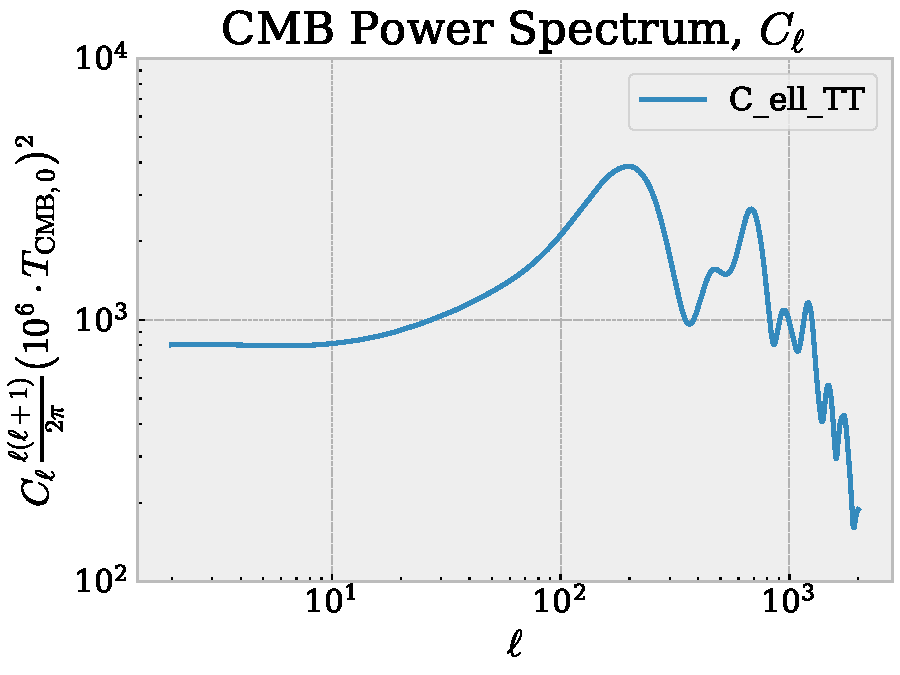
\includegraphics[scale=0.5]{../figs/Cells_toy.pdf}
    \caption{Resulting CMB power spectrum using the toy-cosmology for testing against figure in project description.}
    \label{fig: Cell toy}
  \end{figure}

  The matter results are shown in \cref{fig: Matter toy}, the upper panel displaying the interesting results as the matter power spectrum and the matter components overplotted. Again the shape of the spectrum is identical to the test case, with the peak being at approximately the exact same place, while the amplitude is a bit higher. 
  \begin{figure}[ht!]
    \centering
    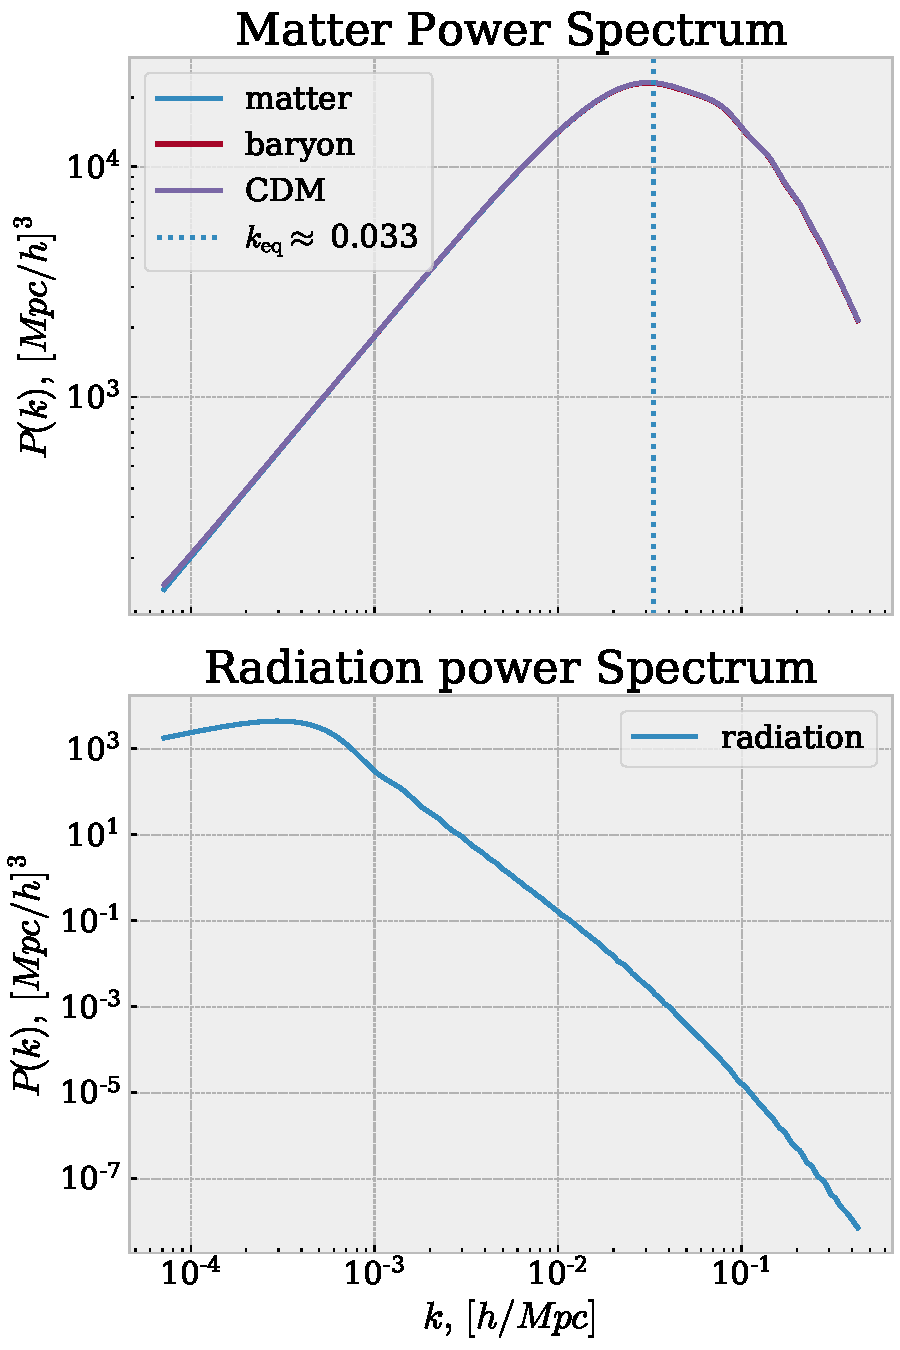
\includegraphics[scale=0.5]{../figs/comp_PS_toy.pdf}
    \caption{Resulting matter power spectrum using the toy-cosmology for testing against figure in project description. Upper panel showing the matter power spectrum, with the spectrum from the components baryons and \rCDM overplotted and the equality scale marked in as the dotted vertical line.}
    \label{fig: Matter toy}
  \end{figure}

\end{appendices}

\end{document}